

\chapter{RootkitArsenal}
\section{Real Mode (chapter 3.3)}
\note[Real mode address space]: Real mode uses 20-bit address space
\begin{note}[Segmented Memory Model]
\begin{center}

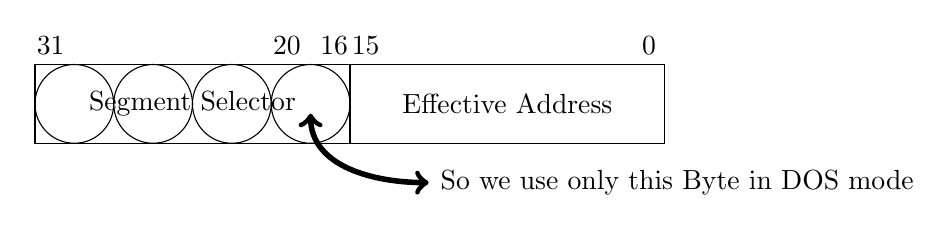
\begin{tikzpicture}
\coordinate [label=above:31] (A) at (0.2,1);
\coordinate [label=above:20] (A) at (3.2,1);
\coordinate [label=above:16] (A) at (3.8,1);
\coordinate [label=above:15] (A) at (4.2,1);
\coordinate [label=above:0] (A) at (7.8,1);
\draw (0,0) rectangle (4,1) node[pos=.5] {Segment Selector};
\draw (4,0) rectangle (8,1) node[pos=.5] {Effective Address};
\foreach \x in {1,2,3,4}
	\draw[baseline] (\x-0.5,0.5 ) node (N\x) {} circle (0.5);
\draw[<->,line width =2pt] [out=-90] (N4)  to [in=180] (5,-0.5) node[right]{So we use only this Byte in DOS mode} ;
\end{tikzpicture}
	
\end{center}
\end{note}

\begin{note}[Registers in real mode]: (p $\rightarrow$ 65)\\
\begin{center}
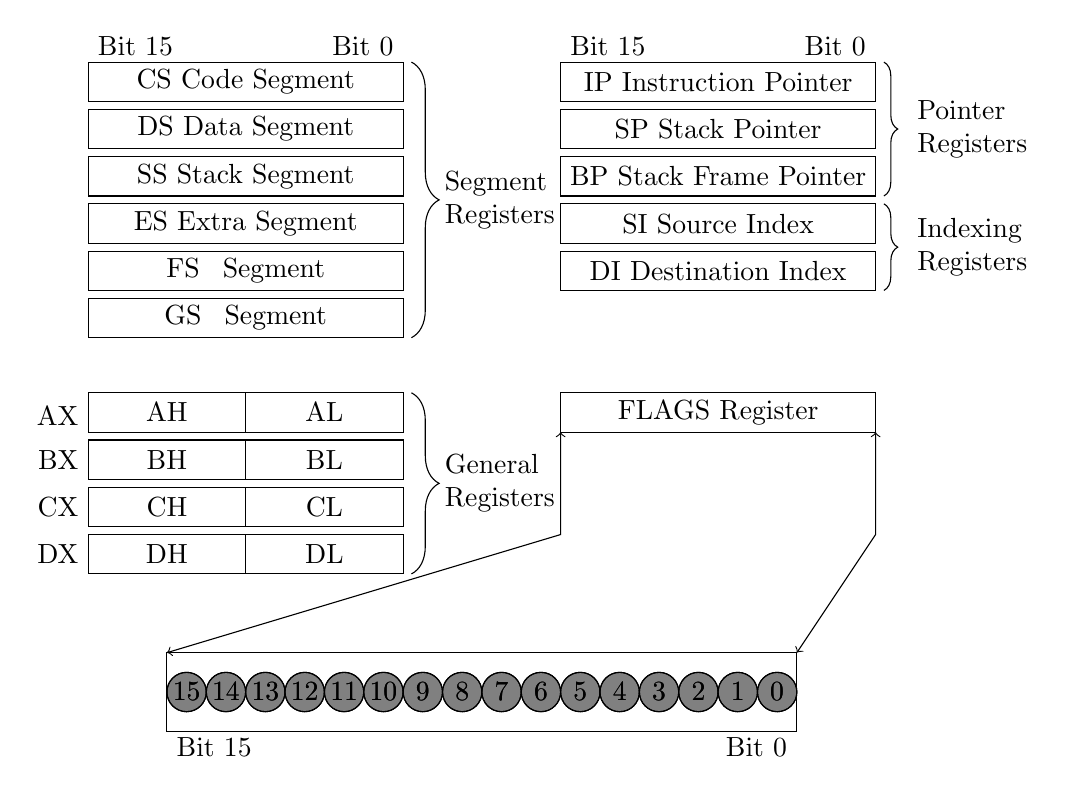
\begin{tikzpicture}
\node[left] at (0,0.25) {DX};
\draw (0,0) rectangle (2,.5) node [pos=0.5] {DH};
\draw (2,0) rectangle (4,.5) node [pos=0.5] {DL};

\node[left] at (0,0.85) {CX};
\draw (0,0.6) rectangle (2,1.1) node [pos=0.5] {CH};
\draw (2,0.6) rectangle (4,1.1) node [pos=0.5] {CL};

\node[left] at (0,1.45) {BX};
\draw (0,1.2) rectangle (2,1.7) node [pos=0.5] {BH};
\draw (2,1.2) rectangle (4,1.7) node [pos=0.5] {BL};

\node[left] at (0,2) {AX};
\draw (0,1.8) rectangle (2,2.3) node [pos=0.5] {AH};
\draw (2,1.8) rectangle (4,2.3) node [pos=0.5] {AL};

\draw [decorate,decoration={brace,amplitude=10pt,mirror},xshift=3pt,yshift=0pt]
(4,0) -- (4,2.3) node [black,midway,right,xshift=0.3cm,text width=1.5cm] 
{General Registers};

\draw (0,3) rectangle (4,3.5) node [pos=0.5] {GS \, Segment};
\draw (0,3.6) rectangle (4,4.1) node [pos=0.5] {FS \, Segment};
\draw (0,4.2) rectangle (4,4.7) node [pos=0.5] {ES Extra Segment};
\draw (0,4.8) rectangle (4,5.3) node [pos=0.5] {SS Stack Segment};
\draw (0,5.4) rectangle (4,5.9) node [pos=0.5] {DS Data Segment};
\draw (0,6) rectangle (4,6.5) node [pos=0.5] {CS Code Segment};

\draw [decorate,decoration={brace,amplitude=10pt,mirror},xshift=3pt,yshift=0pt]
(4,3) -- (4,6.5) node [black,midway,right,xshift=0.3cm,text width=1.5cm] 
{Segment Registers};

\node [right] at (0,6.7) {Bit 15};
\node [left] at (4,6.7) {Bit 0};

\draw (6,1.8) rectangle (10,2.3) node [pos=0.5] {FLAGS Register};

\draw (6,3.6) rectangle (10,4.1) node [pos=0.5] {DI Destination Index};
\draw (6,4.2) rectangle (10,4.7) node [pos=0.5] {SI Source Index};
\draw (6,4.8) rectangle (10,5.3) node [pos=0.5] {BP Stack Frame Pointer};
\draw (6,5.4) rectangle (10,5.9) node [pos=0.5] {SP Stack Pointer};
\draw (6,6) rectangle (10,6.5) node [pos=0.5] {IP Instruction Pointer};
\draw [decorate,decoration={brace,amplitude=5pt,mirror},xshift=3pt,yshift=0pt]
(10,4.8) -- (10,6.5) node [black,midway,right,xshift=0.3cm,text width=1.5cm] 
{Pointer Registers};
\draw [decorate,decoration={brace,amplitude=5pt,mirror},xshift=3pt,yshift=0pt]
(10,3.6) -- (10,4.7) node [black,midway,right,xshift=0.3cm,text width=1.5cm] 
{Indexing Registers};

\node [right] at (6,6.7) {Bit 15};
\node [left] at (10,6.7) {Bit 0};

\draw (1,-1) rectangle (9,-2);
\draw[<->] (6,1.8) -- (6,0.5) -- (1,-1);
\draw[<->] (10,1.8) -- (10,0.5) -- (9,-1);

\foreach \x in {15,...,0}
	\ifthenelse{9 = \x \OR  8 = \x}
	{\draw[fill=gray] (8-\x/2+.75,-1.5) node (B\x) {\x} circle (0.25);}
	{\draw (8-\x/2+.75,-1.5) node (B\x) {\x} circle (0.25);};

	
\node [right] at (1,-2.2) {Bit 15};
\node [left] at (9,-2.2) {Bit 0};
\end{tikzpicture}
\end{center}

\begin{itemize}
\item Bit 8 of FLAGS Register (TF Trap Flag): if this bit is set, the processor generates a single-step interrupt after each instruction. Debuggers use this to single-step through a program.
\item Bit 9 of FLAGS Register (IF Interrupt Enabled Flag): If it is set, then interrupts are enabled.
\end{itemize}
\end{note}

\begin{note}[Real-Mode Interrupts]
\begin{enumerate}
\item An interrupt is some event that triggers the execution of a special kind type of procedure called an \textit{interrupt service routine (ISR)}, also known as an \textit{interrupt handler}
\item In real mode, the first kilobyte of memory (address 0x00000 to 0x003FF) is occupied by \textit{interrupt vector table (IVT)}. In protected mode this structure is called \textit{interrupt descriptor table (IDT)}.
\item The logical address of each ISR in IVT is stored sequentially. like figure \ref{figRootKitRealModeIVT}.
\begin{center}
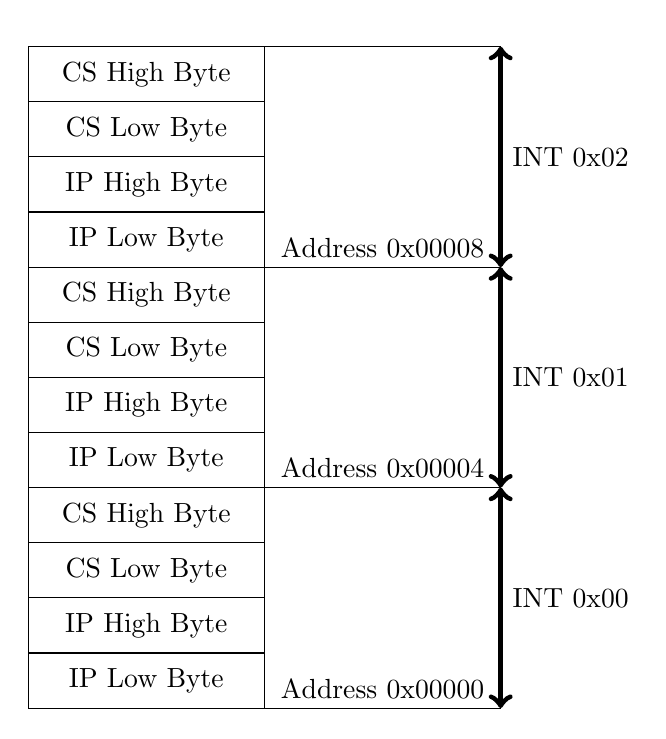
\begin{tikzpicture}
\label{figRootKitRealModeIVT}
\foreach \x in {0,2.8,5.6}
{
	\draw (0,\x) rectangle (3,\x+0.7) node [pos=0.5] {IP Low Byte};
	\draw (0,\x + 0.7) rectangle (3,\x+1.4) node [pos=0.5] {IP High Byte};	
	\draw (0,\x + 1.4) rectangle (3,\x+2.1) node [pos=0.5] {CS Low Byte};	
	\draw (0,\x + 2.1) rectangle (3,\x+2.8) node [pos=0.5] {CS High Byte};		
}
\draw (3,0) -- (6,0) node [pos = 0.5,above] {Address 0x00000};
\draw (3,2.8) -- (6,2.8) node [pos = 0.5,above] {Address 0x00004};
\draw (3,5.6) -- (6,5.6) node [pos = 0.5,above] {Address 0x00008};
\draw (3,8.4) -- (6,8.4) node [pos = 0.5,above] {};

\draw[<->, line width = 2pt] (6,0) -- (6,2.8) node [pos=0.5,right] {INT 0x00};
\draw[<->,line width = 2pt] (6,2.8) -- (6,5.6) node [pos=0.5,right] {INT 0x01};
\draw[<->,line width = 2pt] (6,5.6) -- (6,8.4) node [pos=0.5,right] {INT 0x02};
\end{tikzpicture}
\end{center}
\item Under MS-DOS, the BIOS handles interrupts 0 through 31, and DOS handles interrupts 32 through 63. the remaining interrupts (64 to 265) are for user-defined interrupts.
\item There are three types of Interrupts
\begin{itemize}
\item Hardware Interrupts (maskable and nonmaskable).
\item Software Interrupts.
\item Exceptions (faults, traps and aborts).
\end{itemize}
Maskbale hardware interrupts can be disabled by clearing IF\footnote{Interrupt Enabled Flag} like interrupt 8 (system timer). Software interrupts (also known as internal interrupts) are implemented in a program using INT instruction. like:
\begin{lstlisting} [language={[x86masm]Assembler}]
mov AH,02H
mov DL,41H
int 21H
\end{lstlisting}
\end{enumerate}
\end{note}

\begin{note}[Different jump types: Short, Near and Far:]\\

\begin{table}[!htbp]
	\makegapedcells
	\centering
	\resizebox{\textwidth}{!}{%resizing the whole table
\begin{tabular}{|c|c|c|}\hline
 \textbf{\textcolor{blue}{JMP Type}} & \textbf{\textcolor{blue}{Example}} & \textbf{\textcolor{blue}{Real Mode Machine Encoding}}  \\[\rowheight] \hline
\textbf{Short} & JMP SHORT mylabel & 0xEB [signed bytes]  \\ [\rowheight] \hline
\textbf{Near direct} & JMP NEAR PTR mylabel & 0xE9 [low byte][high byte]  \\ [\rowheight] \hline
\textbf{Near indirect} & JMP BX & 0xFF 0xE3  \\ [\rowheight] \hline
\textbf{Far direct} & JMP DS:[mylabel] & 0xEA [IP low][IP high][CS low][CS high]  \\ [\rowheight] \hline
\textbf{Far indirect} & JMP DWORD PTR [BX] & 0xFF 0x2F  \\ [\rowheight] \hline
 \textbf{\textcolor{blue}{CALL Type}} & \textbf{\textcolor{blue}{Example}} & \textbf{\textcolor{blue}{Real Mode Machine Encoding}}  \\[\rowheight] \hline
\textbf{Near direct} & CALL mylabel & 0xE8 [low byte][high byte]  \\ [\rowheight] \hline
\textbf{Near indirect} & CALL BX & 0xFF 0xD3  \\ [\rowheight] \hline
\textbf{Far direct} & CALL DS:[mylabel] & 0x9A [IP low][IP high][CS low][CS high]  \\ [\rowheight] \hline
\textbf{Far indirect} & CALL DWORD PTR [BX] & 0xFF 0x1F  \\ [\rowheight] \hline
\textbf{Near return} & RET & 0xC3  \\ [\rowheight] \hline
\textbf{Far return} & RETF & 0xCB  \\ [\rowheight] \hline
\end{tabular}
}
\caption{Jump and call tables}
\end{table}
\end{note}
\newpage
\section{Protected Mode (P.87)}
\begin{note}[Dedicated-purpose registers for protected mode]\\
\begin{center}
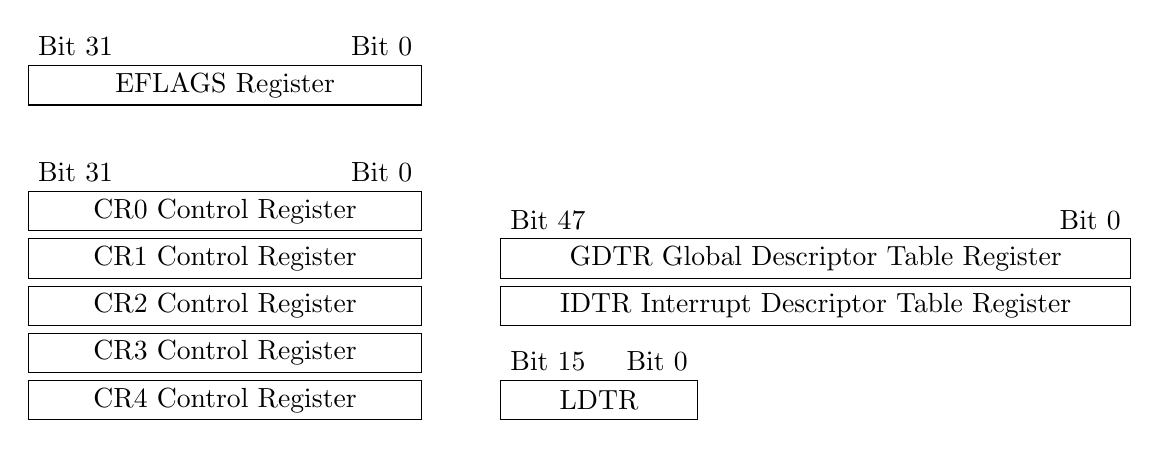
\begin{tikzpicture}
\draw (0,0) rectangle (5,0.5) node [pos=0.5] {CR4 Control Register};
\draw (0,0.6) rectangle (5,1.1) node [pos=0.5] {CR3 Control Register};
\draw (0,1.2) rectangle (5,1.7) node [pos=0.5] {CR2 Control Register};
\draw (0,1.8) rectangle (5,2.3) node [pos=0.5] {CR1 Control Register};
\draw (0,2.4) rectangle (5,2.9) node [pos=0.5] {CR0 Control Register};
\node at (0,2.9) [above right] {Bit 31};
\node at (5,2.9) [above left] {Bit 0};

\draw (0,4) rectangle (5,4.5) node [pos=0.5] {EFLAGS Register};
\node at (0,4.5) [above right] {Bit 31};
\node at (5,4.5) [above left] {Bit 0};

\draw (6,0) rectangle (8.5,0.5) node [pos=0.5] {LDTR};
\node at (6,0.5) [above right] {Bit 15};
\node at (8.5,0.5) [above left] {Bit 0};

\draw (6,1.2) rectangle (14,1.7) node [pos=0.5] {IDTR Interrupt Descriptor Table Register};
\draw (6,1.8) rectangle (14,2.3) node [pos=0.5] {GDTR Global Descriptor Table Register};
\node at (6,2.3) [above right] {Bit 47};
\node at (14,2.3) [above left] {Bit 0};
\end{tikzpicture}
\end{center}
\begin{itemize}
\item Of the six segment registers (CS,DS,ES,FS,GS,SS), the CS register is the only one that cannot be set explicitly. Instead, the CS Register contents must be set implicitly through instructions that transfer program control (JMP,CALL,INT,RET,IRET,SYSENTER,SYSEXIT,etc)
\end{itemize}
\end{note}

\begin{note}[Protected-Mode Segmentation]
\begin{itemize}
\item Paging is an optional feature but segmentation is mandatory.
\item There are two types of descriptor tables, GDT \footnote{Global Descriptor Table}  and LDT \footnote{Local Descriptor Table} , GDT is mandatory.
\remark \normalfont The first entry in GDT is always empty and is referred to as a \textit{null segment descriptor}. A selector that refers to this descriptor in the GDT is called \textit{null selector}.
\end{itemize}
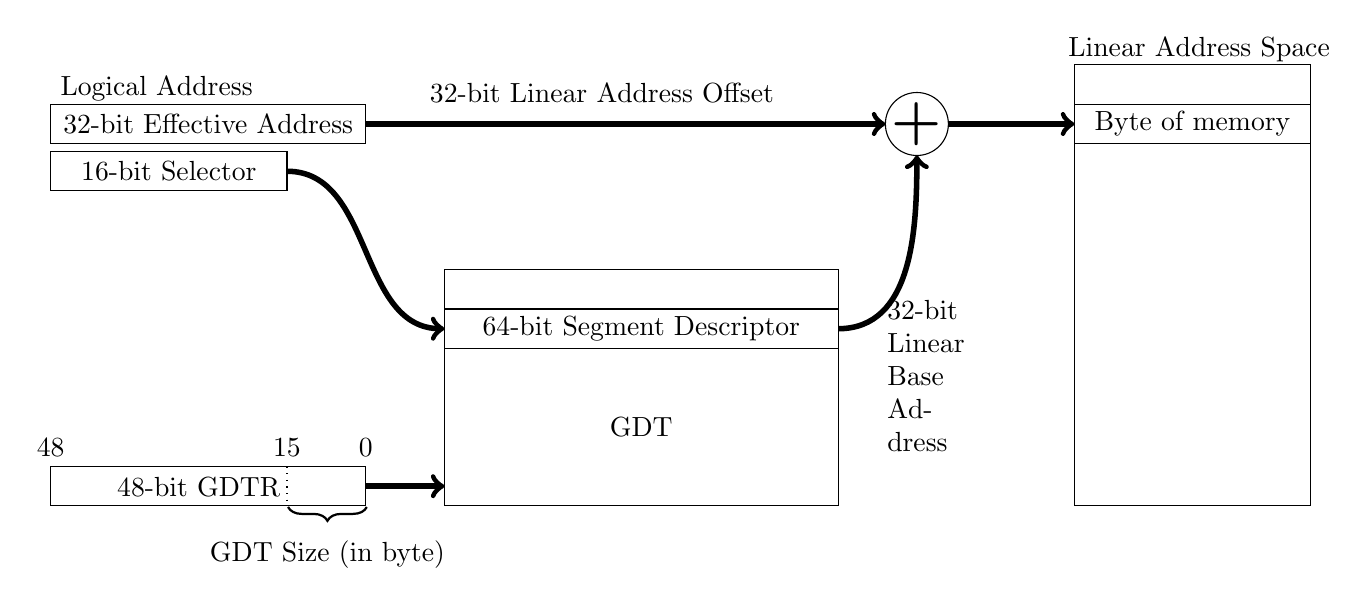
\begin{tikzpicture}
\draw (0,0) rectangle (4,0.5) node [pos=0.47] {48-bit GDTR};
\draw [thick,decorate,decoration={brace,amplitude=5pt,mirror},xshift=0.4pt,yshift=-0.4pt](3,0) -- (4,0) node[black,midway,yshift=-0.6cm] {GDT Size (in byte)};
\draw node at (0,0.5) [above] {48};
\draw node at (4,0.5) [above] {0};
\draw[dotted] (3,0.5) node [above] {15} -- (3,0);

\draw (5,0) rectangle (10,2) node [pos=0.5] {GDT};
\draw (5,2) rectangle (10,2.5) node [pos=0.5] {64-bit Segment Descriptor};
\draw (5,2.5) rectangle (10,3);

\draw (0,4) rectangle (3,4.5) node [pos=0.5] {16-bit Selector};
\draw (0,4.6) rectangle (4,5.1) node [pos=0.5] {32-bit Effective Address};
\draw node at (0,5.3) [above, right] {Logical Address} ;

\draw[->, line width = 2pt] [out = 0] (3,4.25) to [in = 180] (5,2.25);
\draw[->, line width = 2pt] [out = 0] (4,0.25) to [in = 180] (5,0.25);

\draw (11,4.85) circle (0.4) node {\textbf{\huge +}};
\draw[->, line width = 2pt] [out = 0] (4,4.85) to [in = 180] (10.6,4.85) ;
\draw node at (7,5) [above] {32-bit Linear Address Offset} ;
\draw[->, line width = 2pt] [out = 0] (10,2.25) to [in = -90] (11,4.45);
\draw node at (10.5,1.65) [right,text width=1.2cm] {32-bit Linear Base Address} ;

\draw (13,0) rectangle (16,4.6);
\draw (13,4.6) rectangle (16,5.1) node [pos=0.5] {Byte of memory};
\draw (13,5.1) rectangle (16,5.6);
\draw node at (12.8,5.8) [above, right] {Linear Address Space} ;
\draw[->, line width = 2pt] [out = 0] (11.4,4.85) to [in = 180] (13,4.85);
\end{tikzpicture}\\

The most 13 valuable bits of the Segment Selector are index into GDT. So there can be only $2^{13} = 8192$ entries, and each entry (Segment Descriptor) is 8 byte long so maximum size of GDT is $2^{13} \times 2^{3} = 2^{16}$ in byte which perfectly fits into GDTR size partition.

\begin{center}
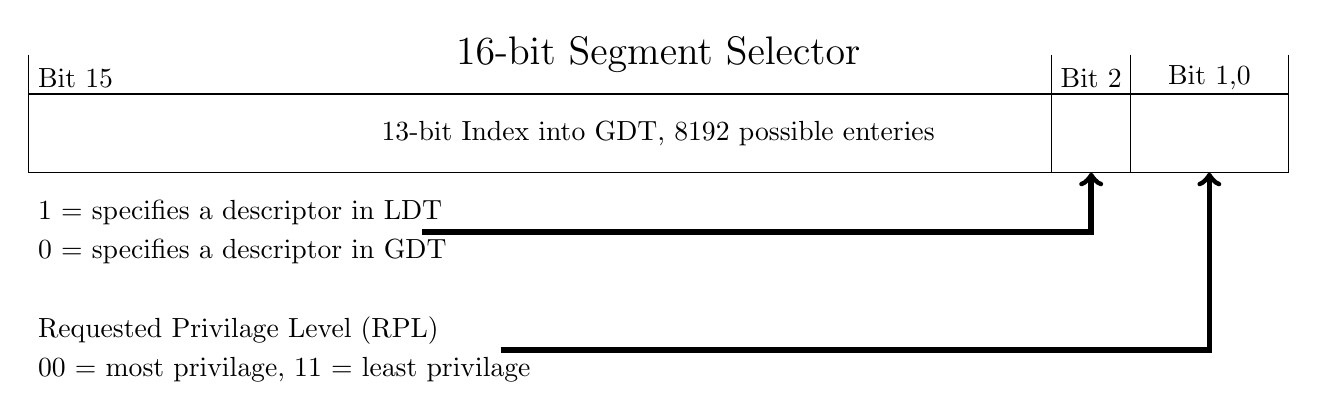
\begin{tikzpicture}
\draw node at (8,1.5) {{\Large 16-bit Segment Selector}};
\draw (0,0)  rectangle (16,1) node [pos=0.5] {13-bit Index into GDT, 8192 possible enteries};
\foreach \x in {16,14,13,0}
\draw (\x,1.5) -- (\x,0);
\draw node at (15,1.2) {Bit 1,0};
\draw node at (13.5,1.2) {Bit 2};
\draw node at (0,1.2) [right] {Bit 15};
\draw node at (0,-0.5) [right] {1 = specifies a descriptor in LDT};
\draw node at (0,-1) [right] {0 = specifies a descriptor in GDT};
\draw node at (0,-2) [right] {Requested Privilage Level (RPL)};
\draw node at (0,-2.5) [right] {00 = most privilage, 11 = least privilage};
\draw[->, line width = 2pt] (5,-0.75) -- (13.5,-0.75) -- (13.5,0);
\draw[->, line width = 2pt] (6,-2.25) -- (15,-2.25) -- (15,0);
\end{tikzpicture}
\end{center}

So the the instruction
\lstinline [language={[x86masm]Assembler}] {mov FS:[30h], 0}
When Linear Base Address referenced by FS is 0x00100000, is to
\lstinline [language={[x86masm]Assembler}] {mov [100030h], 0}. Note that in this design, some over allowed Linear Addresses can be generated, for example if Effective Address was 0x20000000 and the Linear Base Address was 0xEFFFFFFF, the result would be greater than 0xFFFFFFFF which is the summit of the 32-bit address space.
\begin{itemize}
\item There are two specific instructions to work with GDTR, The LGDT loads a value into GDTR and the SGDT reads the value stored in GDTR.
\item RPL \footnote{Requested Privilege Level} is stored in Segment Selectors, DPL \footnote{Descriptor Privilege Level} is kept in Segment Descriptors.A Segment with a DPL of 0 is referred to as existing inside of Ring 0. The CPL or \textit{Current Privilege Level} is the value of RPL in the CS and SS Registers.
\end{itemize}
\begin{center}
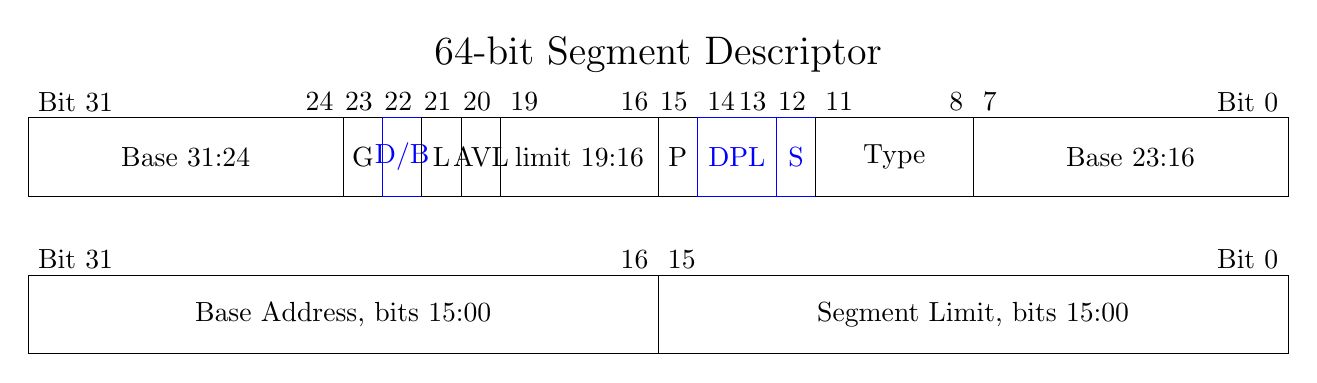
\begin{tikzpicture}
\draw node at (8,3.8) {{\Large 64-bit Segment Descriptor}};
\draw (0,2)  rectangle (4,3) node [pos=0.5] {Base 31:24}; \draw node at (0,3.2) [right] {Bit 31};
\draw (4,2)  rectangle (4.5,3) node [pos=0.5] {G}; \draw node at (4,3.2) [left] {24};
\draw [blue] (4.5,2)  rectangle (5,3) node [pos=0.5] {D/B};\draw node at (4.5,3.2) [left] {23};
\draw (5,2)  rectangle (5.5,3) node [pos=0.5] {L};\draw node at (5,3.2) [left] {22};
\draw (5.5,2)  rectangle (6,3) node [pos=0.5] {AVL}; \draw node at (5.5,3.2) [left] {21};
\draw (6,2)  rectangle (8,3) node [pos=0.5] {limit 19:16}; \draw node at (6,3.2) [left] {20}; \draw node at (6,3.2) [right] {19};
\draw (8,2)  rectangle (8.5,3) node [pos=0.5] {P}; \draw node at (8,3.2) [left] {16};
\draw [blue] (8.5,2)  rectangle (9.5,3) node [pos=0.5] {DPL};\draw node at (8.5,3.2) [left] {15}; \draw node at (8.5,3.2) [right] {14};
\draw [blue] (9.5,2) rectangle (10,3) node [pos=0.5] {S};\draw node at (9.5,3.2) [left] {13};
\draw (10,2)  rectangle (12,3) node [pos=0.5] {Type}; \draw node at (10,3.2) [left] {12}; \draw node at (10,3.2) [right] {11};
\draw (12,2)  rectangle (16,3) node [pos=0.5] {Base 23:16};\draw node at (12,3.2) [left] {8};
\draw (0,0)  rectangle (8,1) node [pos=0.5] {Base Address, bits 15:00};\draw node at (12,3.2) [right] {7};
\draw (8,0)  rectangle (16,1) node [pos=0.5] {Segment Limit, bits 15:00};
\draw node at (16,1.2) [left] {Bit 0};
\draw node at (8,1.2) [right] {15};
\draw node at (8,1.2) [left] {16};
\draw node at (0,1.2) [right] {Bit 31};
\draw node at (16,3.2) [left] {Bit 0};
\end{tikzpicture}

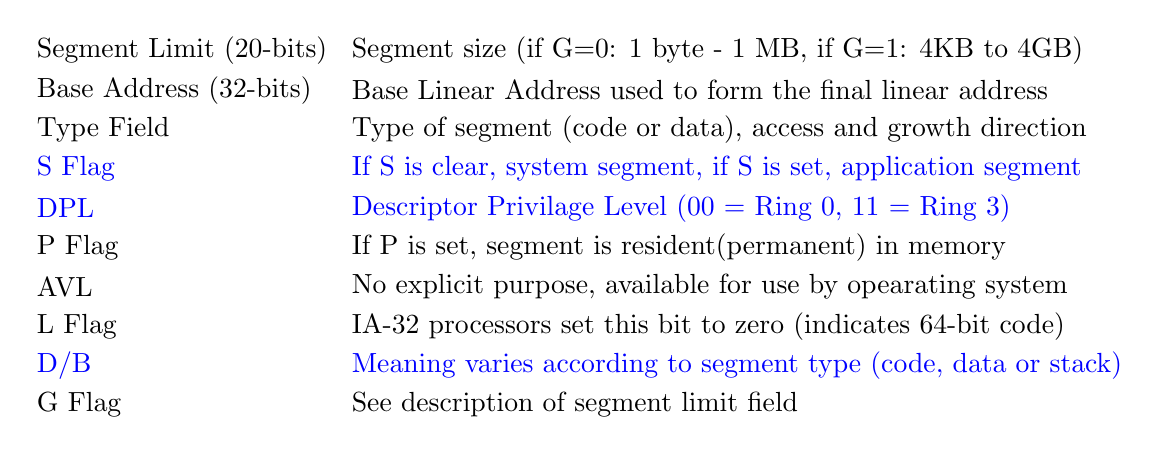
\begin{tikzpicture}
\draw node at (0,-0.5) [right] {Segment Limit (20-bits)};
\draw node at (0,-1) [right] {Base Address (32-bits)};
\draw node at (0,-1.5) [right] {Type Field};
\draw [blue] node at (0,-2) [right] {S Flag};
\draw [blue] node at (0,-2.5) [right] {DPL};
\draw node at (0,-3) [right] {P Flag};
\draw node at (0,-3.5) [right] {AVL};
\draw node at (0,-4) [right] {L Flag};
\draw [blue] node at (0,-4.5) [right] {D/B};
\draw node at (0,-5) [right] {G Flag};

\draw node at (4,-0.5) [right] {Segment size (if G=0: 1 byte - 1 MB, if G=1: 4KB to 4GB)};
\draw node at (4,-1) [right] {Base Linear Address used to form the final linear address};
\draw node at (4,-1.5) [right] {Type of segment (code or data), access and growth direction};
\draw [blue] node at (4,-2) [right] {If S is clear, system segment, if S is set, application segment};
\draw [blue] node at (4,-2.5) [right] {Descriptor Privilage Level (00 = Ring 0, 11 = Ring 3)};
\draw node at (4,-3) [right] {If P is set, segment is resident(permanent) in memory};
\draw node at (4,-3.5) [right] {No explicit purpose, available for use by opearating system};
\draw node at (4,-4) [right] {IA-32 processors set this bit to zero (indicates 64-bit code)};
\draw [blue] node at (4,-4.5) [right] {Meaning varies according to segment type (code, data or stack)};
\draw node at (4,-5) [right] {See description of segment limit field};
\end{tikzpicture}
\end{center}
\end{note}

\begin{note}[Protected-Mode Paging]
\begin{itemize}
\item Each page can be 4KB, 2MB or 4MB in size.
\item If a program references a byte in a page of memory that's currently stored on disk, the processor will generate a \textit{page fault \#PF} exception.
\item The slot in physical memory which pages will be loaded into is called a \textit{page frame}.
\item 32-bit linear address under paging
\begin{center}
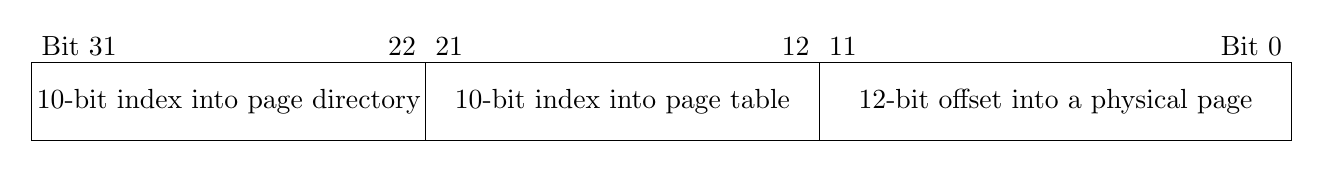
\begin{tikzpicture}
\draw (0,0) rectangle (5,1) node [pos=0.5] {10-bit index into page directory};
\draw (5,0) rectangle (10,1) node [pos=0.5] {10-bit index into page table};
\draw (10,0) rectangle (16,1) node [pos=0.5] {12-bit offset into a physical page};
\draw node at (0,1.2) [right] {Bit 31};
\draw node at (5,1.2) [left] {22};
\draw node at (5,1.2) [right] {21};
\draw node at (10,1.2) [left] {12};
\draw node at (10,1.2) [right] {11};
\draw node at (16,1.2) [left] {Bit 0};
\end{tikzpicture}
\end{center}
\item The physical address (not the linear address) of the first entry of the \textit{page directory} is stored in control register \textbf{CR3}.
\item Each PDE \footnote{Page Directory Entry} contains the base physical address (not the linear address) of a secondary array structure known as the \textit{page table}.
\item Each PTE \footnote{Page Table Entry} contains the physical address of a page of memory.
\end{itemize}
\begin{center}
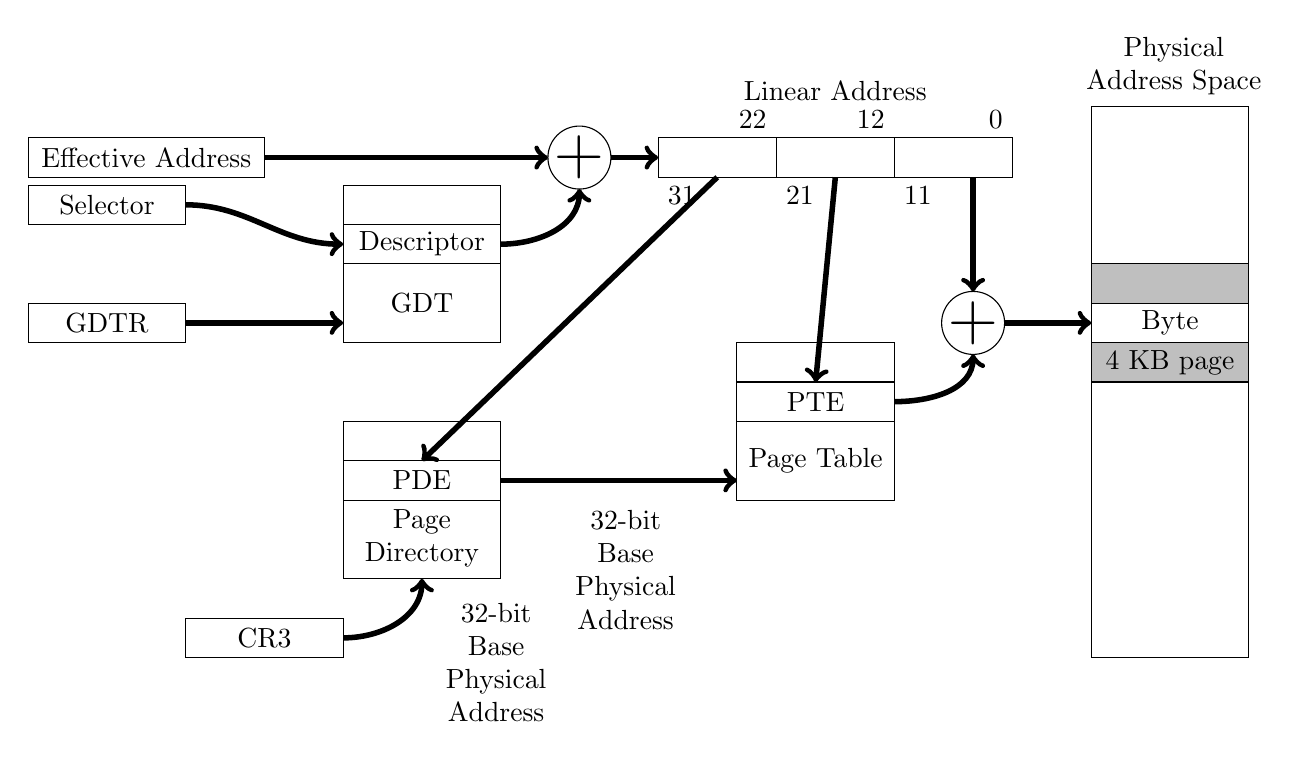
\begin{tikzpicture}
\draw (2,0) rectangle (4,0.5) node [pos=0.5] {CR3};
\draw[->,line width = 2pt] [out=0] (4,0.25) to [in = -90](5,1) node [label={[align=center]-45:32-bit \\Base \\Physical\\ Address}] {};
\draw (4,1) rectangle (6,2) node [label={[align=center,xshift=-1.0cm, yshift=-1.1cm]Page\\Directory}] {};
\draw (4,2) rectangle (6,2.5) node [pos = 0.5] {PDE};
\draw[->,line width=2pt] (6,2.25) -- (9,2.25) node [label={[align=center,label distance = 0.5cm]-160:32-bit \\Base \\Physical\\ Address}] {};
\draw (4,2.5) rectangle (6,3);

\draw (0,4) rectangle (2,4.5) node [pos=0.5] {GDTR};
\draw [->,line width = 2pt] (2,4.25) to (4,4.25);
\draw (4,4) rectangle (6,5) node [pos=0.5] {GDT};
\draw (4,5) rectangle (6,5.5) node [pos = 0.5] {Descriptor};
\draw [->,line width = 2pt,out = 0] (6,5.25) to [in = -90] (7,5.95);
\draw (4,5.5) rectangle (6,6);

\draw (0,5.5) rectangle (2,6) node [pos=0.5] {Selector};
\draw [->,line width = 2pt,out = 0] (2,5.75) to [in = 180] (4,5.25);
\draw (0,6.1) rectangle (3,6.6) node [pos=0.5] {Effective Address};
\draw [->,line width = 2pt] (3,6.35) to (6.6,6.35);
\draw (7,6.35) circle (0.4) node {\Huge +};
\draw [->,line width = 2pt] (7.4,6.35) to (8,6.35);

\draw (8,6.1) node [below right] {31} rectangle (9.5,6.6) node [above left] {22};
\draw [->,line width = 2pt] (8.75,6.1) to (5,2.5);
\draw (9.5,6.1) node [below right] {21} rectangle (11,6.6) node [above left] {12};
\draw [->,line width = 2pt] (10.25,6.1) to (10,3.5);
\draw (11,6.1) node [below right] {11} rectangle (12.5,6.6) node [above left] {0};
\draw node at (10.25,7.2) {Linear Address};

\draw (9,2) rectangle (11,3) node [pos=0.5] {Page Table};
\draw (9,3) rectangle (11,3.5) node [pos = 0.5] {PTE};
\draw (9,3.5) rectangle (11,4);

\draw (13.5,0) rectangle (15.5,3.5);
\draw[fill=lightgray] (13.5,3.5) rectangle (15.5,4) node [pos=0.5] {4 KB page};
\draw (13.5,4) rectangle (15.5,4.5) node [pos=0.5] {Byte};
\draw[fill=lightgray] (13.5,4.5) rectangle (15.5,5);
\draw (13.5,4.5) rectangle (15.5,7);
\draw node at (14.25,7.5) [label={[align=center,xshift=0.3cm,yshift=-0.6cm]Physical \\Address Space}] {};

\draw (12,4.25) circle (0.4) node {\Huge +};
\draw [->,line width = 2pt] (12,6.1) to (12,4.65);
\draw [->,line width = 2pt] (12.4,4.25) to (13.5,4.25);
\draw [->,line width = 2pt, out = 0] (11,3.25) to [in = -90] (12,3.85);
\end{tikzpicture}
\end{center}

With the described routine of paging, we are restricted to 4GB of memory ($1024 \times 1024 \times 4096 = 4GB$). But with the assistive method of PAE\footnote{Paging with Address Extension} we can extend the limit up to 52 address lines.
\end{note}

\begin{note}[Paging with Address Extension (PAE)]
\begin{enumerate}
\item There is a PAE flag in CR4 which PAE is enabled if that flag is set.
\item With PAE enabled, the linear address is broken into four parts instead of just three.
\begin{center}
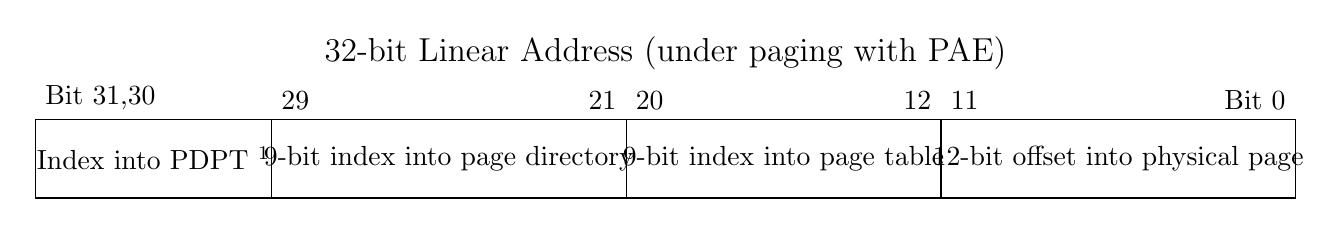
\begin{tikzpicture}
\draw (0,0) rectangle (3,1) node [pos = 0.5] {Index into PDPT \footnote{Page Directory Pointer Table}};
\draw (3,0) rectangle (7.5,1) node [pos = 0.5] {9-bit index into page directory};
\draw (7.5,0) rectangle (11.5,1) node [pos = 0.5] {9-bit index into page table};
\draw (11.5,0) rectangle (16,1) node [pos = 0.5] {12-bit offset into physical page};
\draw node at (0,1) [above right] {Bit 31,30};
\draw node at (3,1) [above right] {29};
\draw node at (7.5,1) [above left] {21};
\draw node at (7.5,1) [above right] {20};
\draw node at (11.5,1) [above left] {12};
\draw node at (11.5,1) [above right] {11};
\draw node at (16,1) [above left] {Bit 0};
\draw node at (8,1.5) [above] {{\large 32-bit Linear Address (under paging with PAE)}};
\end{tikzpicture}
\end{center}
\item Paging with PAE maps a 32-bit linear address to a 52-bit physical address. If a particular IA-32 processor has less than 52 address lines, the corresponding higher order bits of each physical address generated will simply set to zero.
\item Take a look at image on P $\rightarrow$ 97
\end{enumerate}
\end{note}

\begin{note}[A Closer Look at the Tables]
\begin{itemize}
\item Both the PDE and PTE are 32-bit structures.
\end{itemize}
\begin{center}
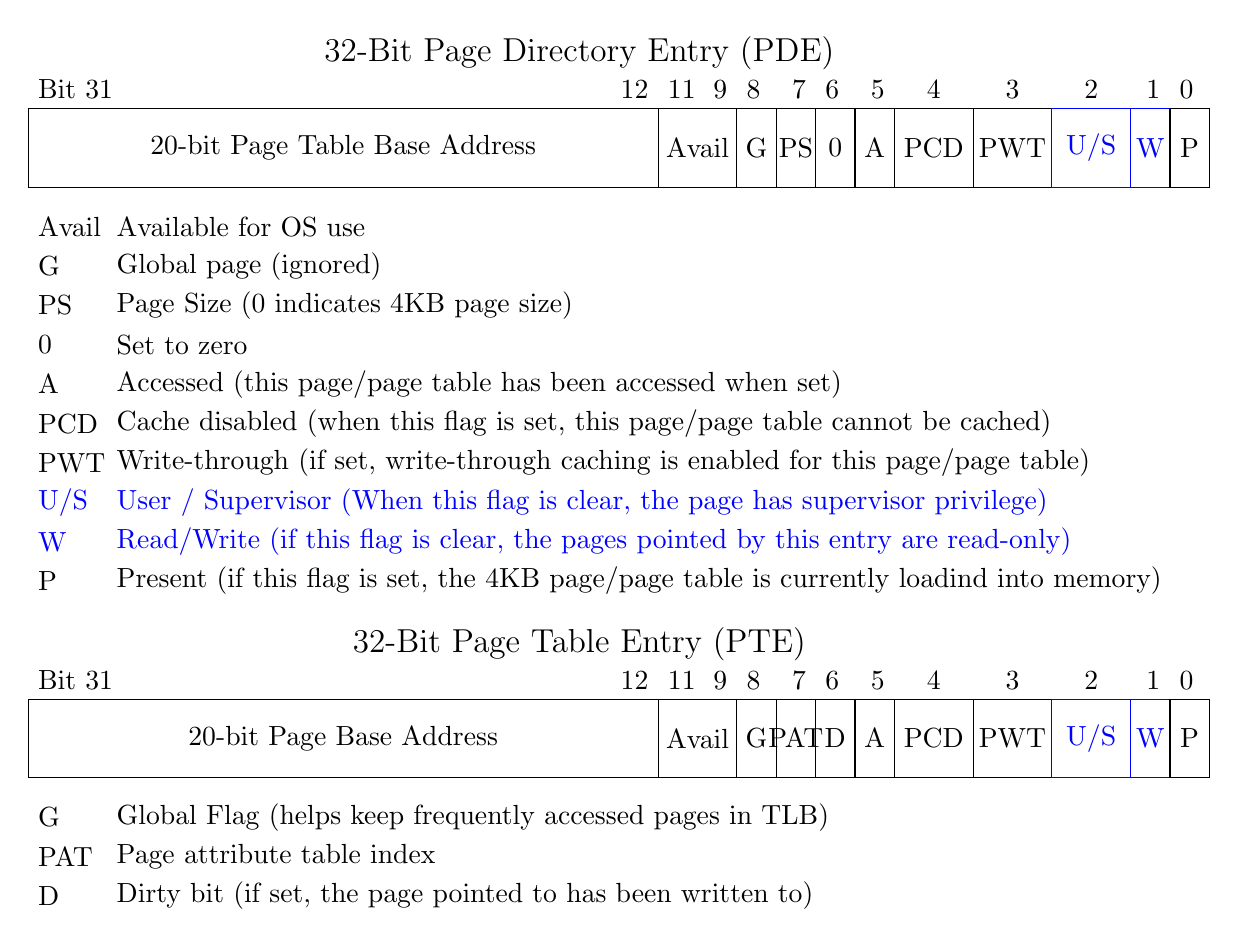
\begin{tikzpicture}
\draw node at (7,1.7) {{\large 32-Bit Page Directory Entry (PDE)}};
\draw (0,0) rectangle (8,1) node [pos = 0.5] {20-bit Page Table Base Address};
\draw (8,0) rectangle (9,1) node [pos = 0.5] {Avail};
\draw (9,0) rectangle (9.5,1) node [pos = 0.5] {G};
\draw (9.5,0) rectangle (10,1) node [pos = 0.5] {PS};
\draw (10,0) rectangle (10.5,1) node [pos = 0.5] {0};
\draw (10.5,0) rectangle (11,1) node [pos = 0.5] {A};
\draw (11,0) rectangle (12,1) node [pos = 0.5] {PCD};
\draw (12,0) rectangle (13,1) node [pos = 0.5] {PWT};
\draw [blue] (13,0) rectangle (14,1) node [pos = 0.5] {U/S};
\draw [blue] (14,0) rectangle (14.5,1) node [pos = 0.5] {W};
\draw (14.5,0) rectangle (15,1) node [pos = 0.5] {P};

\draw node at (0,1) [above right] {Bit 31};
\draw node at (8,1) [above left] {12};
\draw node at (8,1) [above right] {11};
\draw node at (9,1) [above left] {9};
\draw node at (9,1) [above right] {8};
\draw node at (10,1) [above left] {7};
\draw node at (10,1) [above right] {6};
\draw node at (11,1) [above left] {5};
\draw node at (11.5,1) [above] {4};
\draw node at (12.5,1) [above] {3};
\draw node at (13.5,1) [above] {2};
\draw node at (14.5,1) [above left] {1};
\draw node at (14.5,1) [above right] {0};

\draw node at (0,-0.5) [right] {Avail};
\draw node at (1,-0.5) [right] {Available for OS use};
\draw node at (0,-1) [right] {G};
\draw node at (1,-1) [right] {Global page (ignored)};
\draw node at (0,-1.5) [right] {PS};
\draw node at (1,-1.5) [right] {Page Size (0 indicates 4KB page size)};
\draw node at (0,-2) [right] {0};
\draw node at (1,-2) [right] {Set to zero};
\draw node at (0,-2.5) [right] {A};
\draw node at (1,-2.5) [right] {Accessed (this page/page table has been accessed when set)};
\draw node at (0,-3) [right] {PCD};
\draw node at (1,-3) [right] {Cache disabled (when this flag is set, this page/page table cannot be cached)};
\draw node at (0,-3.5) [right] {PWT};
\draw node at (1,-3.5) [right] {Write-through (if set, write-through caching is enabled for this page/page table)};
\draw [blue] node at (0,-4) [right] {U/S};
\draw [blue] node at (1,-4) [right] {User / Supervisor (When this flag is clear, the page has supervisor privilege)};
\draw [blue] node at (0,-4.5) [right] {W};
\draw [blue] node at (1,-4.5) [right] {Read/Write (if this flag is clear, the pages pointed by this entry are read-only)};
\draw node at (0,-5) [right] {P};
\draw node at (1,-5) [right] {Present (if this flag is set, the 4KB page/page table is currently loadind into memory)};

\draw node at (7,-5.8) {{\large 32-Bit Page Table Entry (PTE)}};
\draw (0,-7.5) rectangle (8,-6.5) node [pos = 0.5] {20-bit Page Base Address};
\draw (8,-7.5) rectangle (9,-6.5) node [pos = 0.5] {Avail};
\draw (9,-7.5) rectangle (9.5,-6.5) node [pos = 0.5] {G};
\draw (9.5,-7.5) rectangle (10,-6.5) node [pos = 0.5] {PAT};
\draw (10,-7.5) rectangle (10.5,-6.5) node [pos = 0.5] {D};
\draw (10.5,-7.5) rectangle (11,-6.5) node [pos = 0.5] {A};
\draw (11,-7.5) rectangle (12,-6.5) node [pos = 0.5] {PCD};
\draw (12,-7.5) rectangle (13,-6.5) node [pos = 0.5] {PWT};
\draw [blue] (13,-7.5) rectangle (14,-6.5) node [pos = 0.5] {U/S};
\draw [blue] (14,-7.5) rectangle (14.5,-6.5) node [pos = 0.5] {W};
\draw (14.5,-7.5) rectangle (15,-6.5) node [pos = 0.5] {P};

\draw node at (0,-6.5) [above right] {Bit 31};
\draw node at (8,-6.5) [above left] {12};
\draw node at (8,-6.5) [above right] {11};
\draw node at (9,-6.5) [above left] {9};
\draw node at (9,-6.5) [above right] {8};
\draw node at (10,-6.5) [above left] {7};
\draw node at (10,-6.5) [above right] {6};
\draw node at (11,-6.5) [above left] {5};
\draw node at (11.5,-6.5) [above] {4};
\draw node at (12.5,-6.5) [above] {3};
\draw node at (13.5,-6.5) [above] {2};
\draw node at (14.5,-6.5) [above left] {1};
\draw node at (14.5,-6.5) [above right] {0};

\draw node at (0,-8) [right] {G};
\draw node at (1,-8) [right] {Global Flag (helps keep frequently accessed pages in TLB)};
\draw node at (0,-8.5) [right] {PAT};
\draw node at (1,-8.5) [right] {Page attribute table index};
\draw node at (0,-9) [right] {D};
\draw node at (1,-9) [right] {Dirty bit (if set, the page pointed to has been written to)};
\end{tikzpicture}
\end{center}
Implicit zeros will be added to each Base Address to turn those into 32-bit addresses.
\end{note}

\begin{note}[A Closer Look at the Control Registers]
\begin{enumerate}
\item If each process is given it's own copy of CR3, as part of its scheduling context, then it would be possible for two process to have the same linear address and yet have that linear address map to a different physical address.
\item CR0's 16th bit is a WP flag (as in write protection). When the WP is set, supervisor level code is not allowed to write into read-only user level memory pages. Whereas this mechanism facilitates the copy-on-write method of process creation (i.e., forking) traditionally used by UNIX systems, this is dangerous to us because it means that a rootkit might not be able to modify certain system data structures.
\end{enumerate}

\begin{center}
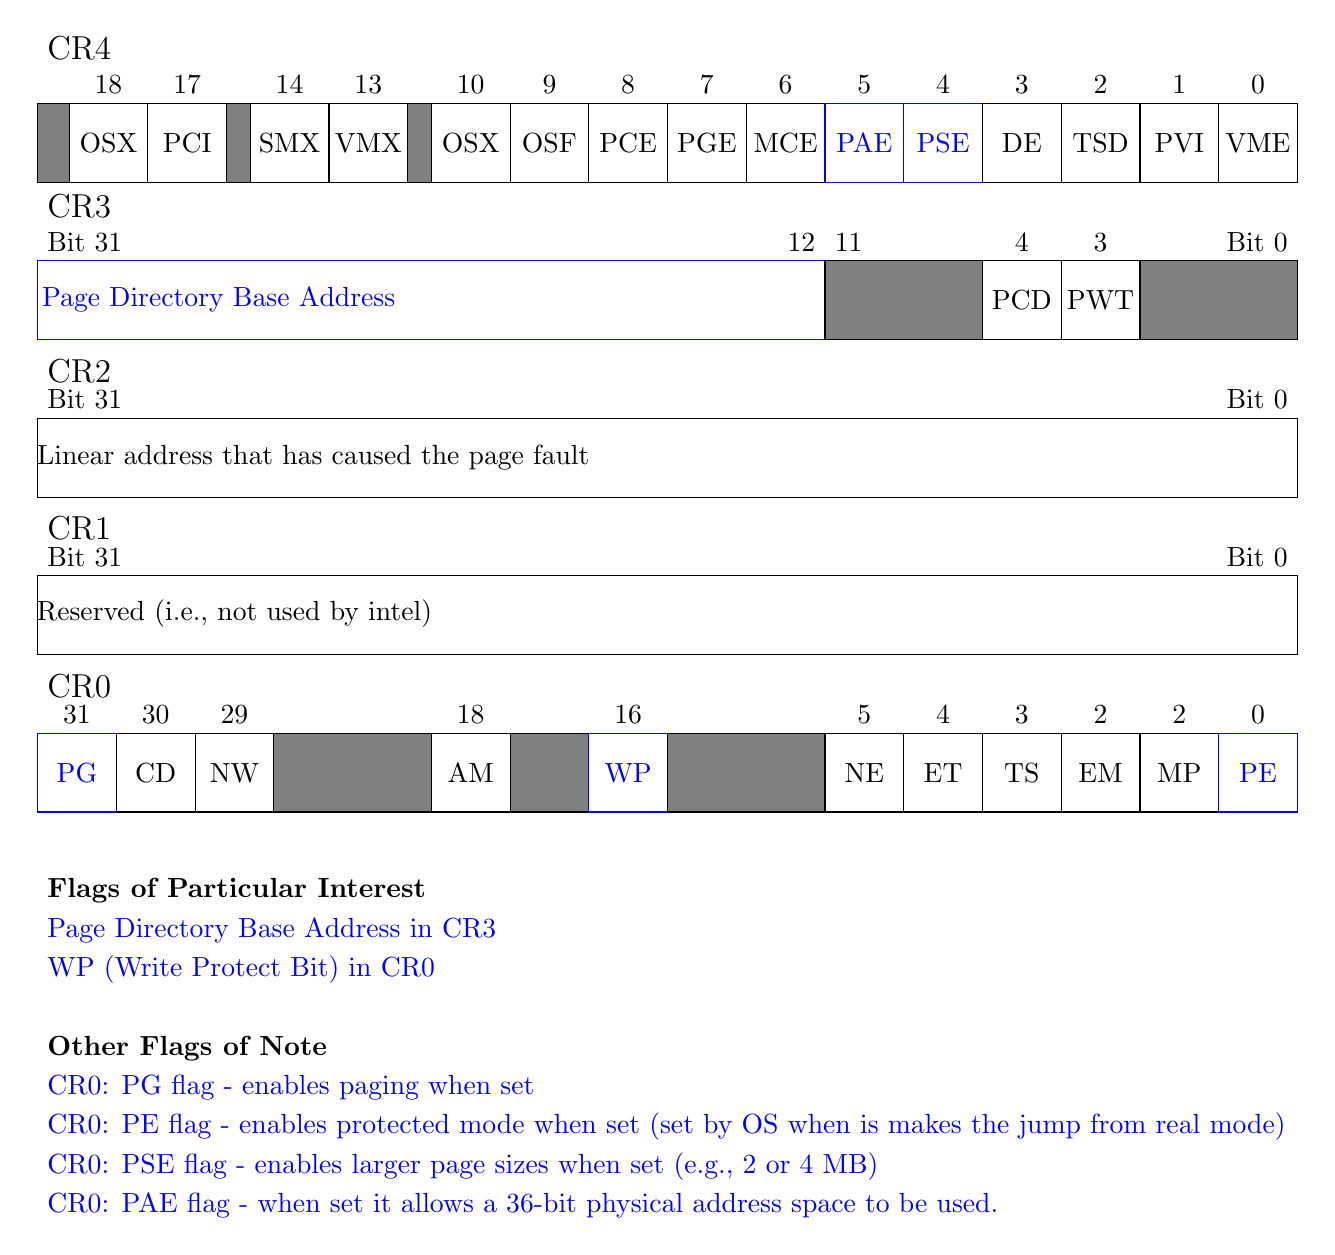
\begin{tikzpicture}
\draw [blue] (0,0) rectangle (1,1) node [pos=0.5] {PG}; \draw node at (0.5,1) [above] {31};
\draw (1,0) rectangle (2,1) node [pos=0.5] {CD}; \draw node at (1.5,1) [above] {30};
\draw (2,0) rectangle (3,1) node [pos=0.5] {NW}; \draw node at (2.5,1) [above] {29};
\draw [fill=gray] (3,0) rectangle (5,1);
\draw (5,0) rectangle (6,1) node [pos=0.5] {AM}; \draw node at (5.5,1) [above] {18};
\draw [fill=gray] (6,0) rectangle (7,1);
\draw [blue] (7,0) rectangle (8,1) node [pos=0.5] {WP}; \draw node at (7.5,1) [above] {16};
\draw [fill=gray] (8,0) rectangle (10,1);
\draw (10,0) rectangle (11,1) node [pos=0.5] {NE}; \draw node at (10.5,1) [above] {5};
\draw (11,0) rectangle (12,1) node [pos=0.5] {ET}; \draw node at (11.5,1) [above] {4};
\draw (12,0) rectangle (13,1) node [pos=0.5] {TS}; \draw node at (12.5,1) [above] {3};
\draw (13,0) rectangle (14,1) node [pos=0.5] {EM}; \draw node at (13.5,1) [above] {2};
\draw (14,0) rectangle (15,1) node [pos=0.5] {MP}; \draw node at (14.5,1) [above] {2};
\draw [blue] (15,0) rectangle (16,1) node [pos=0.5] {PE}; \draw node at (15.5,1) [above] {0};
\draw node at (0,1.6) [right] {\large CR0};

\draw (0,2) rectangle (16,3) node [label={[align=center,xshift=-13.5cm, yshift=-0.9cm] Reserved (i.e., not used by intel)}] {};
\draw node at (0,3) [above right] {Bit 31};
\draw node at (16,3) [above left] {Bit 0};
\draw node at (0,3.6) [right] {\large CR1};

\draw (0,4) rectangle (16,5) node [label={[align=center,xshift=-12.5cm, yshift=-0.9cm] Linear address that has caused the page fault}] {};
\draw node at (0,5) [above right] {Bit 31};
\draw node at (16,5) [above left] {Bit 0};
\draw node at (0,5.6) [right] {\large CR2};

\draw [blue] (0,6) rectangle (10,7) node [label={[align=center,xshift=-7.7cm, yshift=-0.9cm] Page Directory Base Address}] {};
\draw [fill=gray] (10,6) rectangle (12,7);
\draw node at (10,7) [above left] {12}; \draw node at (10,7) [above right] {11};
\draw (12,6) rectangle (13,7) node [pos=0.5] {PCD}; \draw node at (12.5,7) [above] {4};
\draw (13,6) rectangle (14,7) node [pos=0.5] {PWT}; \draw node at (13.5,7) [above] {3};
\draw [fill=gray] (14,6) rectangle (16,7);
\draw node at (0,7) [above right] {Bit 31};
\draw node at (16,7) [above left] {Bit 0};
\draw node at (0,7.7) [right] {\large CR3};

\draw [fill=gray] (0,8) rectangle (0.4,9);
\draw (0.4,8) rectangle (1.4,9) node [pos=0.5] {OSX}; \draw node at (0.9,9) [above] {18};
\draw (1.4,8) rectangle (2.4,9) node [pos=0.5] {PCI}; \draw node at (1.9,9) [above] {17};
\draw [fill=gray] (2.4,8) rectangle (2.7,9);
\draw (2.7,8) rectangle (3.7,9) node [pos=0.5] {SMX}; \draw node at (3.2,9) [above] {14};
\draw (3.7,8) rectangle (4.7,9) node [pos=0.5] {VMX}; \draw node at (4.2,9) [above] {13};
\draw [fill=gray] (4.7,8) rectangle (5,9);
\draw (5,8) rectangle (6,9) node [pos=0.5] {OSX}; \draw node at (5.5,9) [above] {10};
\draw (6,8) rectangle (7,9) node [pos=0.5] {OSF}; \draw node at (6.5,9) [above] {9};
\draw (7,8) rectangle (8,9) node [pos=0.5] {PCE}; \draw node at (7.5,9) [above] {8};
\draw (8,8) rectangle (9,9) node [pos=0.5] {PGE}; \draw node at (8.5,9) [above] {7};
\draw (9,8) rectangle (10,9) node [pos=0.5] {MCE}; \draw node at (9.5,9) [above] {6};
\draw [blue] (10,8) rectangle (11,9) node [pos=0.5] {PAE}; \draw node at (10.5,9) [above] {5};
\draw [blue] (11,8) rectangle (12,9) node [pos=0.5] {PSE}; \draw node at (11.5,9) [above] {4};
\draw (12,8) rectangle (13,9) node [pos=0.5] {DE}; \draw node at (12.5,9) [above] {3};
\draw (13,8) rectangle (14,9) node [pos=0.5] {TSD}; \draw node at (13.5,9) [above] {2};
\draw (14,8) rectangle (15,9) node [pos=0.5] {PVI}; \draw node at (14.5,9) [above] {1};
\draw (15,8) rectangle (16,9) node [pos=0.5] {VME}; \draw node at (15.5,9) [above] {0};
\draw node at (0,9.7) [right] {\large CR4};

\draw node at (0,-1) [right] {\textbf{Flags of Particular Interest}};
\draw [blue] node at (0,-1.5) [right] {Page Directory Base Address in CR3};
\draw [blue] node at (0,-2) [right] {WP (Write Protect Bit) in CR0};
\draw node at (0,-3) [right] {\textbf{Other Flags of Note}};
\draw [blue] node at (0,-3.5) [right] {CR0: PG flag - enables paging when set};
\draw [blue] node at (0,-4) [right] {CR0: PE flag - enables protected mode when set (set by OS when is makes the jump from real mode)};
\draw [blue] node at (0,-4.5) [right] {CR0: PSE flag - enables larger page sizes when set (e.g., 2 or 4 MB)};
\draw [blue] node at (0,-5) [right] {CR0: PAE flag - when set it allows a 36-bit physical address space to be used.};
\end{tikzpicture}
\end{center}
\end{note}